\documentclass[tikz,border=12pt]{standalone}
\usepackage[T1]{fontenc}
\usepackage{tgheros}
\usepackage{sfmath}
\usepackage{amsmath}
% % \usepackage{fontawesome5} (Removed for publication-grade academic typography) (Removed for publication-grade academic typography)
\usepackage{tikz}
\usetikzlibrary{arrows.meta,positioning,shapes.geometric,fit,backgrounds,calc}
\usepackage{xcolor}

\renewcommand{\familydefault}{\sfdefault}

% Neutral Professional Academic Palette
\definecolor{darkslate}{HTML}{0F172A}
\definecolor{bodytext}{HTML}{334155}
\definecolor{mutedtext}{HTML}{64748B}
\definecolor{cardbg}{HTML}{FFFFFF}
\definecolor{subtlebg}{HTML}{F8FAFC}
\definecolor{bordergray}{HTML}{94A3B8}
\definecolor{lightborder}{HTML}{CBD5E1}
\definecolor{linegray}{HTML}{475569}

\begin{document}
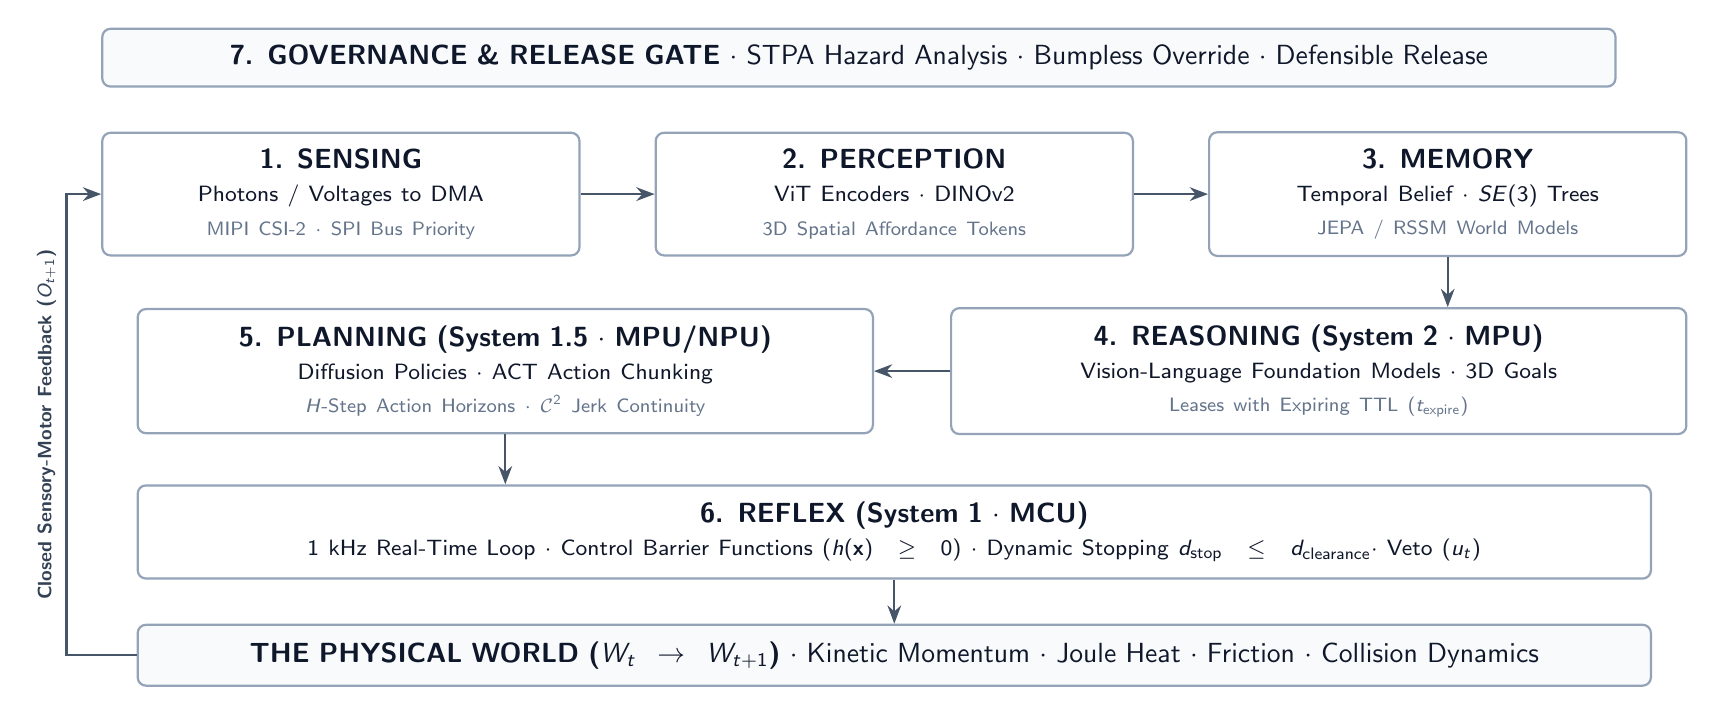
\begin{tikzpicture}[
  font=\sffamily,
  >=Stealth,
  neutralorgan/.style={
    draw=bordergray,
    fill=cardbg,
    rounded corners=3pt,
    line width=0.8pt,
    inner sep=6pt,
    align=center,
    text=darkslate
  },
  neutralarrow/.style={
    ->,
    line width=0.8pt,
    draw=linegray
  }
]

  % Top Banner: Governance & Release Gate
  \node[neutralorgan, text width=7.4in, fill=subtlebg, draw=bordergray] (s7) {
    \textbf{\color{darkslate} 7. GOVERNANCE \& RELEASE GATE} $\cdot$ STPA Hazard Analysis $\cdot$ Bumpless Override $\cdot$ Defensible Release
  };

  % --- TOP ROW: Organs 1, 2, 3 ---
  \node[neutralorgan, text width=2.22in, below=0.22in of s7.south west, anchor=north west] (s1) {
    \textbf{\color{darkslate} 1. SENSING}\\
    {\footnotesize Photons / Voltages to DMA}\\
    {\scriptsize\color{mutedtext}MIPI CSI-2 $\cdot$ SPI Bus Priority}
  };

  \node[neutralorgan, text width=2.22in, right=0.37in of s1] (s2) {
    \textbf{\color{darkslate} 2. PERCEPTION}\\
    {\footnotesize\mbox{ViT Encoders} $\cdot$ \mbox{DINOv2}}\\
    {\scriptsize\color{mutedtext}3D Spatial Affordance Tokens}
  };

  \node[neutralorgan, text width=2.22in, right=0.37in of s2] (s3) {
    \textbf{\color{darkslate} 3. MEMORY}\\
    {\footnotesize Temporal Belief $\cdot$ $SE(3)$ Trees}\\
    {\scriptsize\color{mutedtext}JEPA / RSSM World Models}
  };

  % --- MIDDLE ROW: Organs 5, 4 ---
  \node[neutralorgan, text width=3.51in, below=0.25in of s3.south east, anchor=north east] (s4) {
    \textbf{\color{darkslate} 4. REASONING (System 2 $\cdot$ MPU)}\\
    {\footnotesize Vision-Language Foundation Models $\cdot$ 3D Goals}\\
    {\scriptsize\color{mutedtext}Leases with Expiring TTL ($t_{\text{expire}}$)}
  };

  \node[neutralorgan, text width=3.51in, left=0.38in of s4] (s5) {
    \textbf{\color{darkslate} 5. PLANNING (System 1.5 $\cdot$ MPU/NPU)}\\
    {\footnotesize Diffusion Policies $\cdot$ \mbox{ACT Action Chunking}}\\
    {\scriptsize\color{mutedtext}$H$-Step Action Horizons $\cdot$ $\mathcal{C}^2$ Jerk Continuity}
  };

  % --- LOWER ROW: Organ 6 ---
  \node[neutralorgan, text width=7.4in, below=0.25in of s5.south west, anchor=north west] (s6) {
    \textbf{\color{darkslate} 6. REFLEX (System 1 $\cdot$ MCU)}\\
    {\footnotesize 1 kHz Real-Time Loop $\cdot$ Control Barrier Functions ($h(\mathbf{x}) \ge 0$) $\cdot$ Dynamic Stopping $d_{\text{stop}} \le d_{\text{clearance}} \cdot$ Veto ($u_t$)}
  };

  % --- PHYSICAL WORLD ROW ---
  \node[neutralorgan, draw=bordergray, fill=subtlebg, text width=7.4in, below=0.22in of s6.south west, anchor=north west] (world) {
    \textbf{\color{darkslate} THE PHYSICAL WORLD ($W_t \to W_{t+1}$)} $\cdot$ Kinetic Momentum $\cdot$ Joule Heat $\cdot$ Friction $\cdot$ Collision Dynamics
  };

  % Connecting Arrows
  \draw[neutralarrow] (s1.east) -- (s2.west);
  \draw[neutralarrow] (s2.east) -- (s3.west);
  \draw[neutralarrow] (s3.south) -- (s3.south |- s4.north);
  \draw[neutralarrow] (s4.west) -- (s5.east);
  \draw[neutralarrow] (s5.south) -- (s5.south |- s6.north);
  \draw[neutralarrow] (s6.south) -- (world.north);

  % Closed-loop feedback from physical world back to sensing
  \draw[neutralarrow] (world.west) -- ++(-0.35in, 0) |- (s1.west) 
    node[pos=0.25, above, rotate=90, font=\sffamily\scriptsize\bfseries, text=bodytext] { Closed Sensory-Motor Feedback ($O_{t+1}$)};

\end{tikzpicture}
\end{document}
